\chapter{Homeostat}\label{ch:anexo1}
Para comprender mejor los fundamentos de la homeostasis se diseñó e implementó un Homeostat en el lenguaje de programación Python siguiendo los fundamentos teóricos descritos en el punto explicativo de la homeostasis en este
mismo documento.

Para ello, se implementó una sencilla red de 4 neuronas totalmente interconectadas. En cada iteración, cada neurona recibe una serie de entradas del resto de neuronas y de ella misma. El peso de estas entradas está definido
por la fuerza de conexión entre ellas. El sumatorio ponderado de estas entradas sobre una neurona determina su salida $s_{i}$.

Al comienzo, los pesos de la fuerza de las conexiones están distribuidos de forma aleatoria dentro de los rangos apropiados $R = [0.5 - \alpha, \alpha + 0.5]$, donde $\alpha$ determina la opresión de la restricción homeostática.
Tras cada iteración, si $s_{i} \in R$, la neurona es estable. Si $s_{i} \notin R$ la neurona ha perdido la estabilidad y se activa el mecanismo de cambio adaptativo.

En cuanto se detecta que una neurona ha salido del rango de estabilidad sus parametros comienzan a variar de forma aleatoria (pero dentro de los limites establecidos para cada parametro) hasta que la neurona vuelve a la estabilidad.

La finalidad de este experimento es la comprobar como al comienzo, las neuronas del sistema se podían encontrarse fuera de los rangos de estabilidad (debido a que al principio sus parametros tienen valores aleatorios), pero tras una
serie de iteraciones todas las neuronas se estabilizan.

En la figura \ref{fig:customHomeostat} podemos ver una gráfica que refleja el funcionamiento del Homeostato. En ella, cada linea de color representa la salida de una de las neuronas que componen el Homeostato. Como podemos observar,
al comienzo, partiendo de valores aleatorios en los parámetros, las salidas son inestables y se encuentran fuera del rango establecido. Podemos observar como la neurona representada con el color verde es la última que se estabiliza. Es interesante
también observar como las neuronas se influyen entre ellas durante este proceso de estabilización. Esto puede verse en el último pico ascendente de la neurona representada con el color verde, el cual provoca un ligero movimiento en la
salida de la neurona representada con el color azul, la cual no llega a desestabilizarse (la neurona verde arrastra a la azul con algunos de sus movimientos). Al cabo de un tiempo, todas las neuronas consiguen estabilizarse dentro
del rango establecido. Una vez estables, sin la existencia de ninguna perturbación que provoque la salida de alguna de ellas de la zona de estabilidad, se mantendrán inmutables indefinidamente.

\begin{figure}[H]
    \centering
    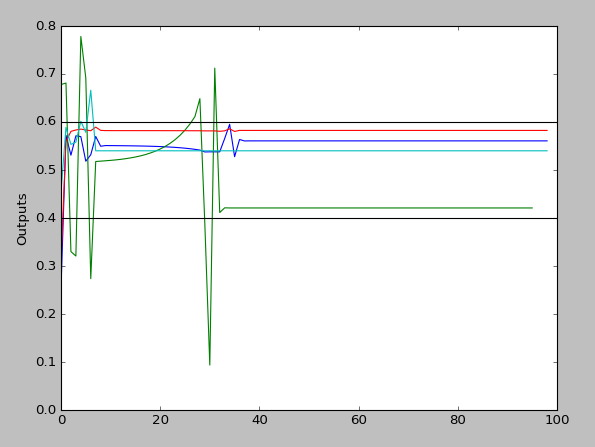
\includegraphics[width=0.8\textwidth,height=8cm]{Imagenes/CustomHomeostat}
    \caption{Gráfica de salidas del Homeostato implementado. \textbf{Eje X:} tiempo. \textbf{Eje Y: } salidas de cada una de las neuronas que componen el Homeostato.}
    \label{fig:customHomeostat}
\end{figure}
